\documentclass[times,utf8,zavrsni]{fer}
\usepackage{booktabs}
\usepackage{tabularx}
\usepackage{listings}
\usepackage{amsmath}
\usepackage{graphicx}



\begin{document}

\thesisnumber{5878}


\title{Računalna statistička analiza jezika religijskih rasprava na internetskim forumima}

\author{Josip Torić}

\maketitle

\zahvala{ Zahvaljujem mentoru izv. prof. dr. sc.~Janu Šnajderu te suradnicima dr. sc.~Mariji Piji Di Buono i dipl. ing.~Mateju Gjurkoviću na motivaciji i savjetima prilikom pisanja ovog rada. \\

Zahvaljujem svojoj majci i svome ocu koji su me uvijek podržavali. \\

Zahvaljujem i svome djedu kojem se ove godine navršava deset godina od smrti. Bez njega ne bih bio čovjek kakav sam danas.
}

\tableofcontents

%%%%%%%%%%%%%%%%%%%%%
\chapter{Uvod}
Ljudi su oduvijek raspravljali o religiji. Religija je sastavni dio života svakog čovjeka, a pri tome je uopće ne bitno je li čovjek religiozan ili nije. Ako je čovjek religiozan, raspravljat će s drugima o svojoj religiji. Ako pak nije religiozan, raspravljat će s drugim ljudima o njihovoj religiji. Ovakvi razgovori su se prije događali na ulici, u trgovima i na sličnim mjestima, no malo je tko mogao prije sto godina zamisliti da će se jedan budist iz Azijske zemlje raspravljati s kršćaninom iz Srednjoeuropske zemlje o religiji, a da se nikad nisu niti će se vjerojatno sresti u životu. Internet nam je omogućio mnogo toga, no najvažnija stvar koju internet omogućava je brzina komunikacije. Komunikacija i razmjena informacije među ljudima nikad u povijesti čovječanstva nije bila ovako brza. Na internetu postoje ogromne količine podataka, a ta količina eksponencijalno raste. Religijske rasprave na internetu su odavno uzele maha, a s količinom podataka koja ostaje kao pisani trag tih rasprava otvaraju se dosad nezamislivi načini spoznavanja vjere i ljudske religije. \\

Cilj rada je analizirati tekstove religijskih rasprava uz pomoć statističke analize. Statistička analiza je širok pojam. Ona obuhvaća sve procese obrade podataka, počevši od prikupljanja podataka pa sve do izvlačenja zaključaka. Statističku analizu dijelimo na deskriptivnu, inferencijalnu i eksplorativnu analizu. Primjenom statistike na jezik, možemo uvidjeti mnoge stvari o jeziku koje nam na prvu možda i nisu očite, tj.~mogli bismo reći da nam statistika omogućava da čitamo između redova. Rezultati koje dobijemo u ovom radu nam mogu pomoći da dublje shvatimo međureligijske odnose te razlike između ponašanja ljudi koji pripadaju različitim religijama.\\

Prvi dio rada odnosi se na opisivanje najvažnijih statističkih metoda. Opisane su deskriptivna statistička analiza, inferencijalna statistička analiza, eksplorativna statistička analiza, frekvencije riječi, značajke LIWC i strojno učenje. Također, u ovom dijelu rada je dan pregled relevantnih radova. Drugi dio rada odnosi se na podatke. Opisan je postupak prikupljanja podataka, obrade podataka te modeliranje podataka za analizu. Treći dio rada odnosi se na rezultate analize. Iznesene su razlike u deskriptivnoj analizi, razlike u vokabularu, razlike u značajkama LIWC, zaključci inferencijalne analize, predikcije logističke regresije te predikcije stroja potpornih vektora. Naposljetku donesen je zaključak o svemu što smo napravili.

%%%%%%%%%%%%%%%%%%%
\chapter{Statistička analiza jezika}
\section{Deskriptivna statistička analiza}
Deskriptivna statistička analiza bavi se mjerama centralne tendencije i mjerama rasipanja. Za razliku od inferencijalne statističke analize, ona ne počiva na teoriji vjerojatnosti. Deskriptivna statistička analiza nam daje jednostavne zaključke o uzorku \citep{openintro}. \\

Najvažnije mjere centralne tendencije su aritmetička sredina, medijan i mod. \\

\subsection{Mjere centralne tendencije}
Aritmetička sredina može se izračunati prema sljedećoj formuli: 
\begin{equation}
\label{mean}
\bar{x}={\frac {x_{1}+x_{2}+\cdots +x_{n}}{n}}
\end{equation}


\noindent gdje ${x_{1}}$ , ${x_{2}}$ , ${\cdots}$, ${x_{n}}$ predstavljaju ${n}$ opservacijskih vrijednosti. Aritmetička sredina populacije, ${\mu}$, predstavlja aritmetičku sredinu izračunatu nad cijelom populacijom te je kao takva rijetko dostupna jer rijetko imamo pristup svim vrijednostima populacije. Aritmetička sredina je statistika uzora i služi kao točkovna procjena ${\mu}$. Aritmetička sredina je osjetljiva na ekstreme, pogotovo ako je uzorak za koji računamo aritmetičku sredinu malen.\\

Medijan je robusna mjera koja predstavlja položajnu srednju vrijednosti koja se nalazi u sredini niza poredanog po veličina. Medijan je neosjetljiv na ekstremen. Medijan se računa prema sljedećoj formuli:
\begin{equation}
\label{median}
M = \begin{cases}
x_{(n+1)/2}, &\text{ako je n neparan}\\
\frac{1}{2}(x_{n/2}+x_{n/2+1}) &\text{ako je n paran}
\end{cases}
\end{equation}



Mod je vrijednost opservacije koja se najčešće pojavljuje. Mod je kao i medijan robusna mjera, tj.~neosjetljiva na ekstreme. \\

U simetričnim distribucijama, mod, medijan i srednja vrijednost su jednaki, dok u zakrivljenim distribucijama srednja vrijednost teži u smjeru zakrivljenosti distribucije. U slučaju zakrivljenih distribucija, medijan je najbolji pokazatelj sredine. Odnos moda, medijana i artimetičke sredine u ovisnosti o zakrivljenosti distribucije možemo vidjeti na slici \ref{fig:meanmedmode}. \\

\begin{figure}[]
	\centering
	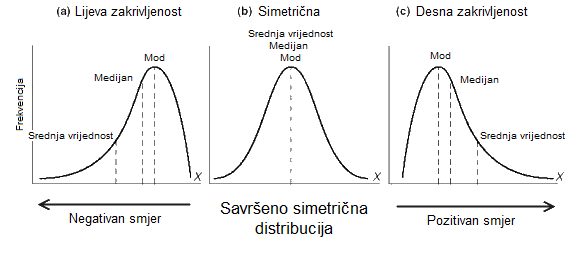
\includegraphics[width=\columnwidth]{img/meanmedianmode.png}
	\caption{Odnos aritmetičke sredine, medijana i mode ovisno o zakrivljenosti distribucije.\protect\footnotemark}
	\label{fig:meanmedmode}
\end{figure}

\footnotetext{Preuzeto sa \url{ https://stats.stackexchange.com/}}

\subsection{Mjere rasipanja}
Najvažnije mjere rasipanja su rang, interkvartilni rang, varijanca, standardna devijacija, i koeficijent varijacije. \\

Rang se računa kao razlika između maksimalne i minimalne vrijednosti. Interkvartilni rang se računa kao razlika između Q1 i Q3. Q1 predstavlja vrijednost koja se nalazi na 25\% niza poredanog po veličina, a Q3 predstavlja vrijednost koja se nalazi na 75\% niza poredanog po veličini. Interkvartilni rang bolje predstavlja rasipanje populacije jer nije osjetljiv na ekstreme. \\

Varijanca ili disperzija populacije predstavlja srednje kvadratno odstupanje populacije od njene srednje vrijednosti. Računa se prema sljedećoj formuli: \\
\begin{equation}
\label{variance}
\sigma ^2=\frac{\sum _{i=0}^N\left(\mu -x_{i}\right)^2}{N}
\end{equation}

\noindent gdje je ${\mu}$ aritmetička sredina populacije, ${x_{i}}$ i-ta opservacija, a N broj članova populacije. \\

Ako nam čitava populacija nije poznata, onda računamo nepristranu procjenu varijance populacije na temelju uzorka od ${n}$ elemenata prema sljedećoj formuli: \\
\begin{equation}
\label{procj}
s ^2=\frac{\sum _{i=0}^N\left(\bar{x} -x_{i}\right)^2}{N-1}
\end{equation}

\noindent gdje je ${\bar{x}}$ aritmetička sredina uzorka, a n broj elemenata uzorka. Iznos ${N-1}$ predstavlja broj stupnjeva slobode pridruženih procjeni varijance. Stupnjevi slobode predstavljaju broj nezavisnih dijelova informacije potrebnih za izračun varijance uzorka. \\

Standardna devijacije uzorka ${\sigma}$ računa se kao korijen iz varijance. Ona nam je važna jer iz nje vrlo lako možemo vidjeti koliko su nam podaci raspršeni. Prema nejednakosti Čebiševa vrijedi da se barem 75\% podataka nalazi unutar 2${\sigma}$ te barem 88,89\% podataka unutar 3${\sigma}$, kao što možemo vidjeti na slici \ref{fig:cebisev}. Ako je pak riječ o podacima koji podilaze normalnoj distribuciji, tada se barem 68\% podataka nalazi unutar 1${\sigma}$, 95\% podataka se nalazi unutar 2${\sigma}$ te 99,73\% podataka se nalazi unutar 3${\sigma}$. Ovo možemo vidjeti na slici \ref{fig:deviation}. \\

\begin{figure}[]
	\centering
	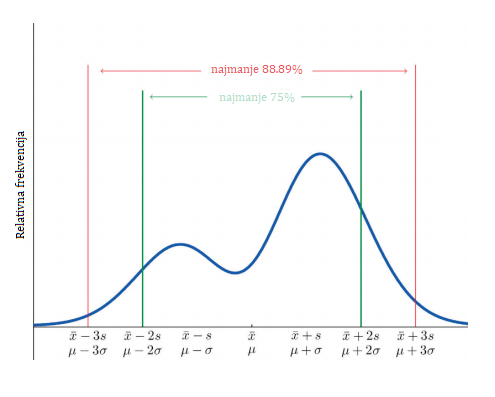
\includegraphics[width=\columnwidth]{img/cebisev.png}
	\caption{Vizualizacija nejednakosti Čebiševa.\protect\footnotemark }
	\label{fig:cebisev}
\end{figure}
\footnotetext{Preuzeto sa \url{https://www.fer.unizg.hr/}}


\begin{figure}[]
	\centering
	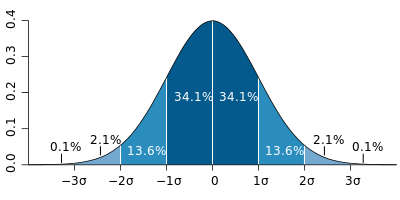
\includegraphics[width=\columnwidth]{img/deviation.png}
	\caption{Standardna devijacija u normalnoj distribuciji.\protect\footnotemark}
	\label{fig:deviation}
\end{figure}
\footnotetext{Preuzeto sa \url{https://en.wikipedia.org/}}

Koeficijent varijacije predstavlja omjer između standardne devijacije i srednje vrijednosti. On nema dimenziju te nam omogućuje usporedbu varijabli izraženih u različitim jedinicama.

%%%%%
\clearpage
\section{Inferencijalna statistička analiza}
Inferencijalna analiza odnosi se na provjeravanje postavljenih hipoteza uz pomoć statističkih testova \citep{openintro}. \\ 

Inferencijalna statistička analiza smije se provoditi samo za distribucije koje odgovaraju normalnoj distribuciji. Ovo se na prvi pogled čini kao prilično limitirajući faktor, no, prema centralnog graničnom teoremu, sve distribucije teže u normalnu distribuciju. Centralni granični teorem kaže ako je $\bar{X}$ aritmetička srednja vrijednost slučajnog uzorka veličine $n$ uzetog iz populacije $s$ s očekivanjem $\mu$ i varijancom $\sigma^2$ onda normirana suma koja se računa prema formuli \ref{cgt} teži po distribuciji u normalnu distribuciju kada $n$ teži u beskonačnost. \\
\begin{equation}
\label{cgt}
Z=\frac{\bar{X}-\mu }{\frac{\sigma }{\sqrt{n}}}
\end{equation}


\noindent Inferencijalna statistička analiza se provodi u nekoliko koraka.\\ 

Prvi korak je postaviti hipoteze. Kod inferencijalne statističke analize imamo dvije hipoteze. Prva hipoteza, ${H_{0}}$ predstavlja nul-hipotezu. nul-hipoteza je hipoteza da ne postoji nikakva značajna razlika između populacija. Druga hipoteza, ${H_{1}}$ predstavlja alternativnu hipotezu. Alternativna hipoteza predstavlja alternativu nultoj hipotezi. \\

Drugi korak je odabrati testnu statistiku. Testna statistika je statistika na temelju čijih se vrijednosti donosi odluka o odbacivanju ili ne odbacivanju zadane osnove statističke hipoteze u korist njezine alternative. Postoji više vrsta testnih statistika, ovisno što želimo testirati u varijablama. \\

Treći korak je odabrati nivo značajnosti $\alpha$ ispod koje ćemo odbaciti nul-hipotezu. Najčešće korištene vrijednosti za nivo značajnosti su 1\% i 5\%. \\

Četvrti korak je izračunati vrijednost statistike i usporediti ga s $\alpha$. Ako je vrijednost statistike manja of $\alpha$, zaključujemo da odbacujemo nul-hipotezu u korist alternativne hipoteze. 


%%%%%%%



\newpage
\section{Eksplorativna statistička analiza}
Eksplorativna statistička analiza za razliku od deskriptivne i inferencijalne analize ne fokusira se na osnovne podatke o podacima i testiranje hipoteza. Eksplorativna analiza se koristi da uvidimo stvari koje nam podaci mogu reći izvan formalnih okvira. \\

Definicija eksplorativne statističke analize glasi: ``Procedure za analizu podataka, tehnike za interpretaciju rezultata, planiranje prikupljanja podataka i svi alati i rezultati statistike koji se mogu primijeniti na podatke" \citep{tukey}. \\

Cilj eksplorativne statistička analiza je istražiti podatke bez definiranih ciljeva u početku te pokušati formulirati sasvim nove hipoteze o podatcima. Eksplorativna statistička analiza nije skup tehnika za analizu podataka već čitav stav kako se treba pristupiti analizi podataka. \\

\begin{figure}[]
	\centering
	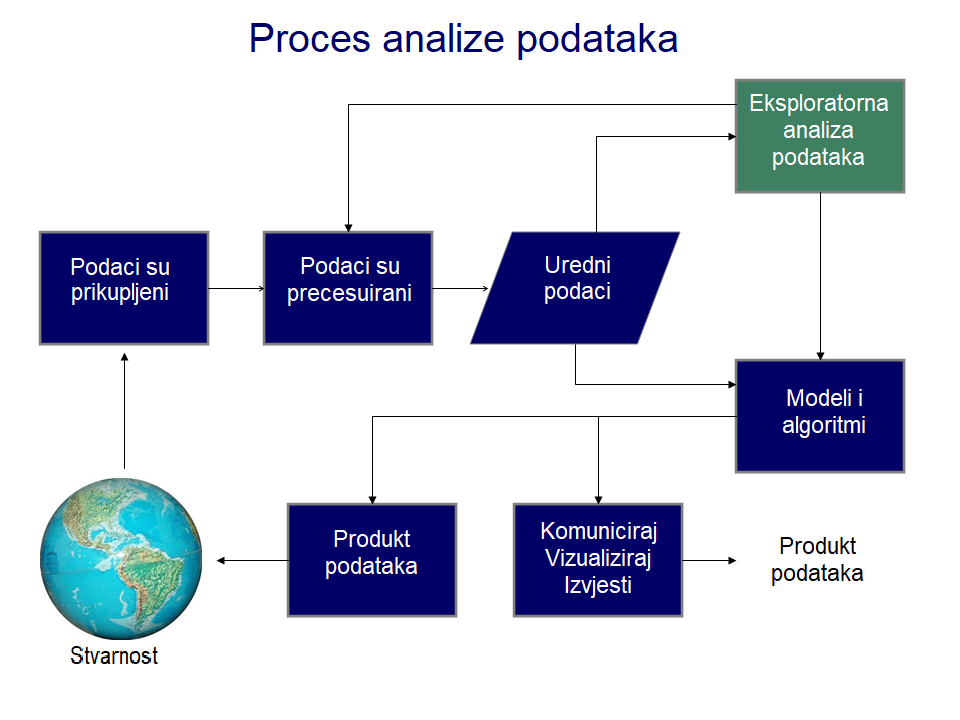
\includegraphics[width=\columnwidth]{img/eda.png}
	\caption{Proces obrade podataka u eksplorativnoj statističkoj analizi.\protect\footnotemark}
	\label{fig:eda}
\end{figure}

\footnotetext{Preuzeto sa \url{https://en.wikipedia.org/}}

\newpage
\section{Značajke LIWC}
LIWC je kratica od Lingvističko ispitivanje i brojanje riječi (engl.~\emph{Linguistic Inquiry and Word Count}). LIWC uzima dani tekst i za svaku značajku LIWC vraća frekvenciju njenog pojavljivanja u tekstu. Značajke LIWC podijeljene su u četiri kategorije: lingvističke varijable, interpunkcijske varijable, ostale gramatičke varijable i psihološke varijable \citep{liwc}. \\

Lingvističke varijable se odnose na dužinu riječi, broj riječi u rečenici, korištenje zamjenica, veznika, pridjeva, negacija i dr. \\

Interpunkcijske varijable odnose se na uporabu točke, zareza, upitnika, uskličnika i ostalih interpunkcijskih znakova. \\

Ostale gramatičke varijable odnose se na uporabu čestih riječi, čestih pridjeva, usporedba, priloga, brojeva i kvantifikatora. \\

Najšira i svakako najzanimljivija kategorija su psihološke varijable. Psihološke varijable nam pokušavaju analitički prikazati psihološko stanje osobe koja je napisala tekst. Psihološke varijable podijeljene su u deset potkategorija: afektivne varijable, socijalne varijable, kognitivne varijable, osjetne varijable, biološke varijable, varijable poriva, vremenske varijable, varijable kretanja i vremena, osobne varijable i varijable neformalnog izražavanja. \\


Za svaku od navedenih varijabli, osim naravno za metričke varijable, LIWC ima u svojem rječniku skup riječi koje predstavljaju tu varijablu. Rječnik se sastoji od gotovo 6400 riječi, a za svaku riječ je definirana jedna ili više kategorija kojoj ta riječ pripada. LIWC zatim prolazi kroz čitav tekst, za svaku varijablu pronalazi koliko riječi u tekstu pripada toj varijabli te naposlijetku za svaku varijablu dijeli broj ponavljanja te varijable s ukupnim brojem riječi u tekstu da bi dobio frekvenciju pojavljivanja te varijable. \\


Prednost LIWC je što na jednostavan i računalno nezahtjevan način možemo saznati razne psihološke stvari o tekstu i osobi koja je napisala tekst. Također, LIWC napreduje kroz godine. Autori istraživanja i samog programa kroz godine povećavaju rječnik koji koriste za kategorizaciju riječi te sami broj kategorija. Prva verzija LIWC koja ja izašla devedesetih godina sadržavala je 80 kategorija i oko 1000 riječi u rječniku, a posljednja verzija u trenutku pisanja ovog teksta je izašla 2015. godine te sadrži 92 varijable i gotovo 6400 riječi u rječniku.


Naravno, i LIWC ima svoje mane. LIWC ne razumije ironiju, sarkazam ili metafore. No, LIWC za svaki tekst izvlači 92 značajke. Ako je netko zloban u korištenju sarkazma, postoji velika vjerojatnost da će LIWC prepoznati njegovu zlobnost u korištenju ostalih riječi u tekstu. Također, LIWC je deskriptivni statistički alat, a kao takav, njegovi rezultati su pouzdaniji ako tekst ima mnogo riječi. Tekst s 10000 riječi će dati mnogo bolje rezultate o tekstu nego tekst od 100 riječi. \\

\newpage
\section{Strojno učenje}
\subsection{Općenito o strojnom učenju}
Strojno učenje je podgrana umjetne inteligencije koja se razvila iz raspoznavanja uzoraka i statistike. Iako strojno učenje zvuči jako komplicirano i futuristički, istina je ipak malo blaža. Definicija glasi: ``Strojno učenje jest programiranje računala tako da optimiziraju neki kriterij uspješnosti temeljem podatkovnih primjera ili prethodnog iskustva" \citep{machine}. Strojno učenje nije ništa drugo nego predviđanje svojstva novih podataka na temelju svojstva starih podataka. \\

Algoritam strojnog učenja pomoću starih podataka stvara model koji je definiran parametrima čije se vrijednosti određuju iz starih podataka, tj.~podataka koje smo ustupili algoritmu. Strojno učenje ima dva problema do kojih može doći prilikom stvaranja modela. Prvi problem je prenaučenost, a do njega dolazi kada je model koji algoritam stvori prekompleksan, tj.~kada ima previše parametara s obzirom na broj podataka te se onda u model ugrade i slučajne značajke podataka, a ne temeljni odnosi između podatcima. Ovo rezultira time da model dobro radi na predviđanju svojstva starih podataka, no na novim podatcima gotovo da uopće i ne radi. Drugi problem je podnaučenost. Do podnaučenosti dolazi kad je model prejednostavan te ne može uopće obuhvatiti temeljne odnose između podatcima u svoje parametre. \\

Strojno učenje dijeli se na nadzirano učenje i nenadzirano učenje. Kod nadziranog učenja podatci su uređeni parovi (ulaz, izlaz)=($x$, $y$), a cilj je pronaći funkciju zavisnosti $y$ o $x$. Ako je $y$ diskretna vrijednost onda govorimo o klasifikaciji podataka, a ako je $y$ kontinuirana vrijednost onda govorimo o regresiji. Kod nenadziranog učenja podatci su bez ciljne vrijednosti, a cilj je naći pravilnost u podatcima. Nenadzirano učenje se dijeli na grupiranje, procjenu gustoće i smanjenje dimenzionalnosti.

%%%%%%%%%55
\subsection{Logistička regresija}
Logistička regresija je metoda za klasifikaciju podataka u diskretne klase. Logistička regresija je takva da predviđa vjerojatnost ishoda kada postoje samo dvije mogućnosti (istina ili laž). Ako želimo logičku regresiju iskoristiti za predviđanje više od dvije mogućnosti, koristit ćemo mulitnomijalnu logističku regresiju. Svaki problem je zasebna klasifikacija u dvije mogućnosti, odnosno da li podatak spada u tu klasu ili ne spada. Za onu klasu za koju dobijemo najveću vjerojatnost da podatak pripada u nju, proglasit ćemo da podatak pripada toj klasi \citep{regression}. \\

Varijabla koju želimo predvidjeti logističkom regresijom mora biti nominalna, dok varijable o kojima želimo da model zavisi moraju biti numeričke. Logistička funkcija definirana je prema sljedećoj formuli:
\begin{equation}
\label{logiFun}
f\left(z\right)=\frac{1}{1+e^{-z}}
\end{equation}


\noindent gdje se varijabla $z$ računa na sljedeći način: \\
\begin{equation}
\label{logiZ}
z=\beta_{0}\:+\beta_{1}x_{1}\:+\beta_{2}x_{2}\:+\:\cdots\:+\:\beta_{n}x_{n}\:=\:\beta +\sum _{n=1}^N\left(B_{i}x_{i}\right)
\end{equation}

\noindent U gornjoj formuli varijable $x_{1}$, $x_{2}$ do $x_{n}$ predstavljaju vrijednost pojedine varijable, a koeficijenti $\beta_{0}$, $\beta_{1}$ do $\beta_{n}$ predstavljaju koje logistička regresija pridodaje pojedinim varijablama. Vrijednosti koeficijenata pronalaze se uz pomoć optimizacijskih tehnika kao što je gradijentni spust.

\begin{figure}[]
	\centering
	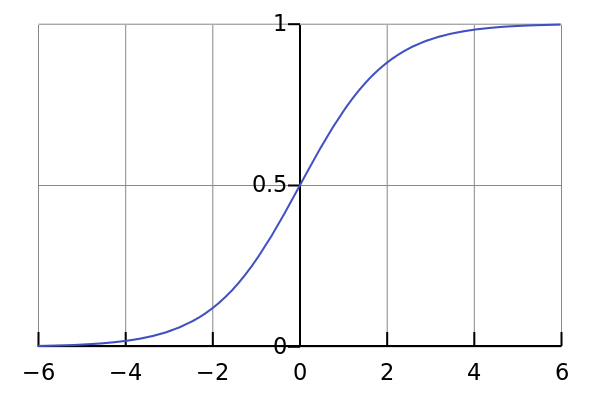
\includegraphics[width=10cm]{img/logistic.png}
	\caption{Graf logističke funkcije.\protect\footnotemark }
	\label{fig:logistic}
\end{figure}

\footnotetext{Preuzeto sa \url{https://en.wikipedia.org/}}

\clearpage


%%%%%%%%%%%%%%
\subsection{Stroj potpornih vektora}
Stroj potpornih vektora jedan je od najpopularnijih modela strojnih učenja koji se danas koristi pri bilo kojoj klasifikaciji. Stroj potpornih vektora je klasifikator koji konstrukcijom hiperravnine u visokodimenzijskom prostoru stvara model koji predviđa kojoj klasi pripada novi uzorak. Stroj potpornih vektora na ulaz dobiva podatke povezane s klasom kojoj pripadaju te ih prikazuje kao točke u prostoru raspoređene na način da su točke koje predstavljaju podatke koji pripadaju različitim klasama međusobno što razmaknutije \citep{learnsvm}. \\

Zadatak stroja potpornog vektora je odabrati optimalnu hiperravninu razdvanja. Optimalna hiperravnina razdvajanja je ona koja ostavlja najviše slobodnog prostora između klasa, tj.~ maksimizira marginu između hiperravnine i klasa. Model koristi vektore podataka za određivanje maksimalne margine i ti vektori se nazivaju potporni vektori. \\

Na slici \ref{fig:logistic} prikazano je kako stroj potpornih vektora odabire optimalnu hiprerravninu razdvajanja. Naime, hiperravnina $H_{1}$ ne razdvaja klase uopće, hiperravnina $H_{2}$ razdvaja klase ali s malom marginom, dok hiperravnina $H_{3}$ razdvaja klase s najvećom marginom. \\

\begin{figure}[]
	\centering
	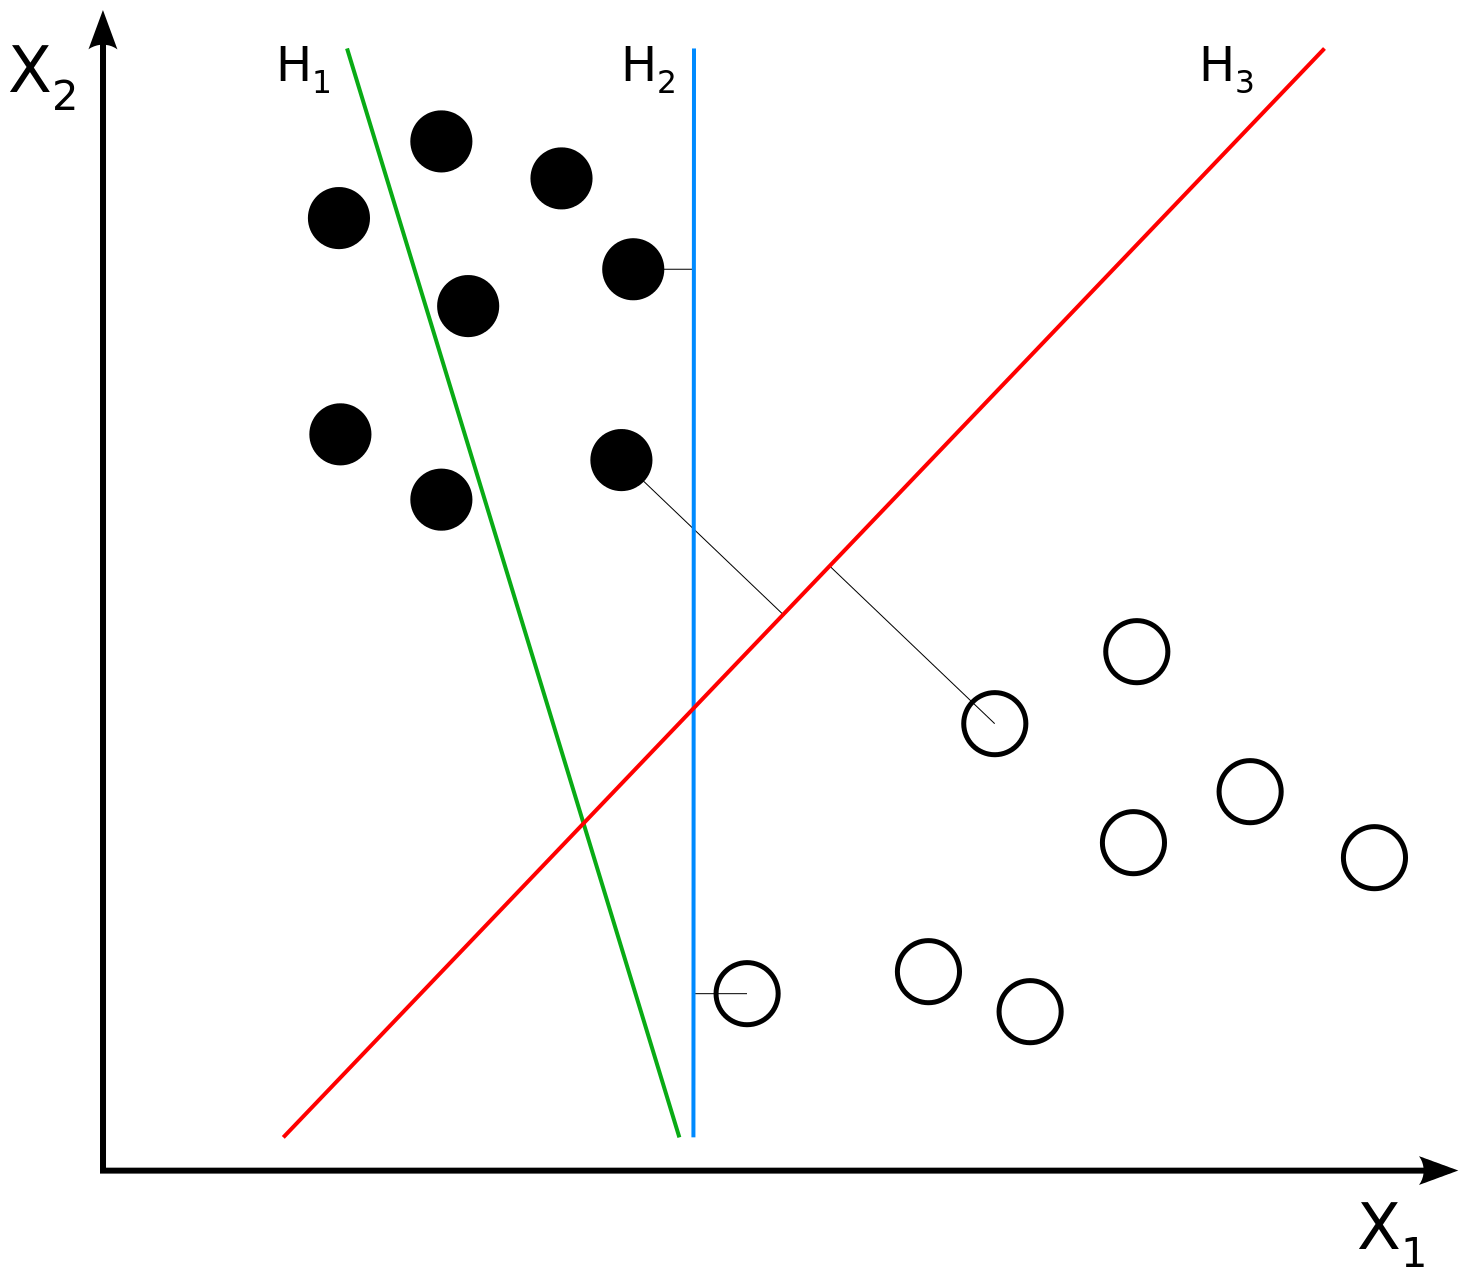
\includegraphics[width=250px]{img/svm.png}
	\caption{Odabir hiperravnine u stroju potpornih vektora.\protect\footnotemark }
	\label{fig:logistic}
\end{figure}

\footnotetext{Preuzeto sa: \url{https://en.wikipedia.org/}}


\newpage
\section{Relevantni radovi}

Relevantnih radova za temu ovog rada nema previše. Nijedan rad nije ušao u temu računalnu statističku lingvističku analizu religijskih rasprava. \\

\citep{rahimi} je u svom radu analizirao odnos jezika i religije u Iranu. Analizirao je religijske tekstove i njihov način pisanja. Također, proučavao je kako različite vrste jezika koji se koriste u religijskim tekstovima utječu na ljude. \\

\citep{darquen} su u svom radu analizirali način na koji religija utječe na formiranje jezika. Opisivali su jezik korišten u najvažnijim vjerskim tekstovima za svaku od pojedinih religija (Biblija, Kuran, Talmud) te način na koji su ti tekstovi utjecali na formiranje jezika pripadnika pojedinih religija. Također, proučavali su način na koji je razvoj jezika utjecao na razvoj religije.



%%%%%%%%%%%%%%%
\chapter{Podaci}


Za obradu podataka i izračun rezultata koristili smo programski jezik R. Programski jezik R je odabran jer podržava veliki broj statističkih funkcija, brz je u radu s velikim skupovima podataka i pogodan za prikazivanje rezultata statističke analize.

%%%
\section{Prikupljanje podataka}
Prikupljanje podataka je prvi i osnovni korak analize podataka. Bez kvalitetnih podataka ne možemo ništa napraviti. \\

Podatke za ovaj rad prikupili smo s društvene mreže Reddit. Reddit je najveća internetska platforma za raspravu. Rasprave su podijeljene po dretvama (engl.~\emph{thread}), a svaka dretva predstavlja neku temu. Postoje dretve o raznim temama kao što su politika, znanost, umjetnost, sport itd. Za religijske rasprave, odabrana je dretva naziva ``debateReligion". Na toj dretvi, korisnici raspravljanju o svim svjetskim religijama na civiliziran način. Civiliziran način komuniciranja na toj dretvi nametnut je od administratora dretve koji imaju mogućnost ukloniti svaki neprimjereni komentar. No, najvažniji razlog zašto je ta dretva odabrana je taj što korisnici na toj dretvi postavljaju svoju korisničku oznaku (engl.~\emph{user flair}) na naziv religije kojoj pripadaju. Ta oznaka je onda vidljiva na svim njihovim komentarima. \\

Zatim smo odabrali 4000 korisnika koji su raspravljali na spomenutoj dretvi te za svakog od njih su preuzeti svi komentari koje su ti korisnici ostavljali na društvenoj mreži Reddit, bez obzira o kojoj se dretvi radilo. Cilj ovoga je da dobijemo podatke koje će predstavljati način govora po religijama u svakodnevnom govoru, bez obzira raspravljali li korisnici o religiji, hrani, filmova itd. \\

%%%
\newpage
\section{Obrada podataka}
Nakon prikupljanja podataka dobili smo tri milijuna komentara. Prva stvar je bilo odbaciti sve podatke koji nam nisu bitni za našu analizu kao što su vrijeme objavljivanja komentara, ocjene komentara i slično. Jedini bitni podatci za daljnju analizu su ime korisnika, oznaka autora i tekst komentara. Druga stvar je bilo spojiti sve komentare istog korisnika u jedan komentar. Nakon spajanja svih komentara u jedan komentar, izbacili sam korisnike koji su ukupno ostavili manje od 100 riječi. U skupu podataka ostalo je ukupno 3733 korisnika. \\

Nakon ovoga slijedio je najbitniji korak u obradi podataka za ovaj rad, a to je standardizacija oznaka. Oznake koje su korisnici unosili su bile u obliku običnog teksta. Tako, npr. imamo kršćane (engl.~\emph{Christian}), kršćane-katolike (engl.~\emph{Christian-Catholic}), katolike (engl.~\emph{Catholic}) itd. , a sve ovo zapravo predstavlja jednu religiju. Oznake smo podijelili u 8 skupina,  sekularni (engl.~\emph{Secular}), kršćani (engl.~\emph{Christian}), muslimani (engl.~\emph{Muslim}), budisti (engl.~\emph{Buddhist}), hindusi (engl.~\emph{Hindu}), židovi (engl.~\emph{Jew}), bivši vjernici (engl \emph{Ex-}) te ostali (engl.~\emph{Other}). Vidimo da imamo dvije specifične skupine, a to su bivši vjernici i ostali. Bivši vjernici predstavljaju sve korisnike koji imaju oznake tipa ``Ex-Christian", ``Ex-Muslim", a ostali predstavljaju sve ostale religije koje ne pripadaju niti pod jednu prije navedenu skupinu oznaka, npr. pastafarijanac (engl.~\emph{Pastafarian}), jedi (engl.~\emph{Jedi}) i slično. \\

Jedini korak koji je preostao je da izbacimo ime korisnika iz podataka jer nam taj podatak nije bitan. Svaki podatak nam sada ima samo dva atributa, oznaku religije i tekst komentara. \\


%%
\newpage
\section{Model podataka}
Nakon obrade podataka u našim podatcima imamo 3733 redaka, svaki redak sadrži oznaku religije i tekst komentara. Sada nam preostaje izgraditi model za daljnju obradu. \\

Najveći problem koji nam se pojavio u modelu podataka je taj da su grupe neravnomjerno raspoređena. Raspoređenost po grupama se može vidjeti u tablici \ref{table:dist}. \\

\begin{table}[h!]
\centering
\caption{Broj korisnika po religijama}
\label{table:dist}
\begin{tabular}{@{}ccc@{}}
\hline
Religija  & Broj korisnika & Postotak \\ 
\hline
\hline
Sekularni & 2228  &  59,68\%                 \\
Kršćani   & 567   & 15,18\%                 \\
Ostali    & 506  & 13,55\% \\
Bivši     & 208  & 5,57\%                   \\
Muslimani & 106  & 2,83\%                   \\
Židovi    & 63   & 1,69\%                  \\
Budisti   & 40   & 1,07\%                  \\
Hindusi   & 15  & 0,40\%                 \\
\hline
\end{tabular}
\end{table}

Iz raspoređenosti po grupama možemo vidjeti da daleko najviše ima sekularnih korisnika, nakon njih slijede kršćani i pripadnici ostalih religija. Sekularni korisnici čine čak 59,68\% korisnika, a prve tri religije po pripadnosti čak 88,43\%. Iz ovoga možemo vidjeti da o religiji daleko najviše raspravljaju ljudi koji uopće nisu religiozni. \\

%
\subsection{Frekvencije riječi}
U model podataka dodat ćemo frekvencije 700 najčešćih riječi koje se pojavljuju u svim komentarima nakon izbacivanja zaustavnih (engl.~\emph{stop}) riječi iz teksta. Odabrali smo upravo 700 riječi jer nam je to povoljan omjer između riječi koje predstavljaju vokabular i računalne složenosti izrade modela. Zaustavne riječi su veznici, zamjenice, brojevi i sve ostale riječi koje nemaju nikakvo značenje osim u danom kontekstu. Prvo ćemo spojiti sve komentare u jedan komentar, izbaciti zaustavne riječi, izbrojati ponavljanje svake riječi te sortirati silazno prema učestalosti. Nakon ovoga smo dobili skup od 700 najčešćih riječi. \\ 

Zatim za svaku od 700 najčešćih riječi dodat ćemo stupac s imenom riječi u naše podatke. Kao vrijednost stupca uzet ćemo frekvenciju ponavljanja te riječi u komentaru. Frekvenciju ćemo računati prema:
\begin{equation}
\label{frekv}
\mathit{frekvencija}\left(\mathit{rijec}\right)=\frac{\text{broj ponavljanja}\left(\mathit{rijec}\right)\text{u komentaru}}{\text{ukupan broj riječi u komentaru}}
\end{equation}

Frekvencije riječi, iako naizgled jednostavan podatak, mogu nam dati uvide koriste li neke religije neke riječi više nego ostale.

%
\subsection{Značajke LIWC}
Značajke LIWC smo dobili uz pomoć programa LIWC2015 \citep{liwc}. Program nam je za svaki uneseni komentar (pri tome mislimo da komentar koji je nastao spajanjem svih korisničkih komentara) dao 92 značajke LIWC. Svaka značajka ima značenje frekvencije pojavljivanja te značajke u tekstu, izraženo u postotcima.



%%%%%%%%%%%%%
\chapter{Rezultati}

\section{Razlike u deskriptivnoj analizi}

Iako jednostavna, deskriptivna analiza nam može reći nekoliko stvari o podatcima. \\

Nakon raspoređivanja komentara po religijama, ali prije gradnje samom modela, izračunali smo prosječan broj riječi po komentara i prosječnu dužinu riječi u slovima. Rezultati su prikazani u tablici \ref{table:desc}. \\

\begin{table}[h!]
\centering
\caption{Broj komentara po korisniku, broj riječi po komentaru i dužina riječi po religijama}
\label{table:desc}
\begin{tabular}{@{}cccc@{}}
\hline
Religija  & Broj komentara & Broj riječi po komentaru & Dužina riječi \\ 
\hline
\hline
Bivši     &  685,80   & 12,06                              & 5,39                    \\
Budisti   &  388,80    & 11,94                              & 5,35                    \\
Hindusi   &  617,40  & 11,82                              & 5,38                   \\
Kršćani   &  498,69   & 12,84                              & 5,38                    \\
Muslimani &  536,65  & 12,99                              & 5,37                    \\
Ostali    &  694,77    & 12,83                              & 5,50                    \\
Sekularni &  823,48  & 12,75                              & 5,38                    \\
Židovi    &  629,33  & 13,00                              & 5,41                    \\

\hline
\end{tabular}
\end{table}


Iz tablice \ref{table:desc} možemo vidjeti da najviše komentara ostavljaju korisnici koji se deklariraju kao sekularni, a najmanje budisti. Isto tako, možemo vidjeti da židovi i muslimani ostavljaju komentare s više riječi od ostalih religija. Također, pripadnici ostalih religija imaju najveću prosječnu dužinu riječi. Već ovdje vidimo da postoje razlike u govoru između religija. Ovi podatci, iako van konteksta, mogu nam reći da židovi i muslimani pišu duže komentare te više elaboriraju svoje tvrdnje, dok pripadnici ostalih religija koriste kompleksnije riječi u svojoj komunikaciji.



\newpage

\section{Razlike u vokabularu}

Vokabular pojedinih religija nam može mnogo toga reći o načinu komuniciranja pripadnika pojedinih religija. Uostalom, prema vokabularu smo izgradili model koji smo koristili u analizi pomoću strojnog učenja. \\

Za svaku religiju smo spojili sve komentare iz te religije u jedan komentar te izbrojali učestalost pojavljivanje svake riječi. Dobivene rezultate smo sortirali i izvukli deset najčešće korištenih riječi po religiji. Rezultati su prikazani u tablici \ref{table:voc}. \\


\begin{table}[h!]
\centering
\caption{Deset najčešće korištenih riječi po religijama}
\label{table:voc}
\begin{tabular}{@{}cc@{}}
\hline
Religija  & Deset najčešće korištenih riječi                                       \\
\hline
\hline
Bivši     & \emph{people}, \emph{good}, \emph{will}, \emph{time}, \emph{well}, \emph{shit}, \emph{pretty}, \emph{thing}, \emph{going}, \emph{fuck}    \\
Budisti   & \emph{people}, \emph{will}, \emph{good}, \emph{time}, \emph{well}, \emph{sure}, \emph{pretty}, \emph{going}, \emph{better}, \emph{thing}  \\
Hindusi   & \emph{people}, \emph{will}, \emph{good}, \emph{india}, \emph{time}, \emph{well}, \emph{pretty}, \emph{better}, \emph{guy}, \emph{indian} \\
Kršćani   & \emph{people}, \emph{good}, \emph{will}, \emph{god}, \emph{time}, \emph{well}, \emph{going}, \emph{pretty}, \emph{sure}, \emph{thing}     \\
Muslimani & \emph{people}, \emph{will}, \emph{good}, \emph{islam}, \emph{time}, \emph{muslim}, \emph{muslims}, \emph{god}, \emph{well}, \emph{allah}  \\
Ostali    & \emph{people}, \emph{good}, \emph{will}, \emph{time}, \emph{well}, \emph{going}, \emph{thing}, \emph{better}, \emph{pretty}, \emph{watch} \\
Sekularni & \emph{people}, \emph{good}, \emph{will}, \emph{time}, \emph{well}, \emph{going}, \emph{thing}, \emph{pretty}, \emph{sure}, \emph{better}  \\
Židovi    & \emph{people}, \emph{jews}, \emph{will}, \emph{good}, \emph{jewish}, \emph{fine}, \emph{god}, \emph{israel}, \emph{thing}, \emph{going}   \\

\hline
\end{tabular}
\end{table}


Iz tablice \ref{table:voc} možemo vidjeti da židovi i muslimani najviše pričaju o svojoj religiji, a hindusi o svojoj državi. Kršćani, sekularni, budisti i pripadnici ostalih religija najčešće koriste religijski neutralne riječi. Iz ovoga se može pretpostaviti da muslimanima i židovima, religija predstavlja centralno mjesto u životu. Židovi i muslimani neće previše ulaziti u rasprave koje nisu vezane za religiju jer ih te stvari vjerojatno ne zanimaju. Veoma zanimljiva stvar je da ljudi koji su nekad bili pripadnici neke od religija koriste psovke mnogo više nego ostali, naime možemo vidjeti da među deset najčešćih riječi pojavile su se čak dvije psovke.



\newpage

\section{Razlike u značajkama LIWC}

Razlike u značajkama LIWC, kao i frekvencije riječi, mogu nam mnogo toga reći o načinu komuniciranja pripadnika pojedinih religija. Također, prema značajkama smo izgradili model za strojno učenje. \\

Za svaku smo religiju spojili komentare i izračunali aritmetičku sredinu značajki LIWC značajki za pojedinu religiju. Nakon toga smo izvukli sedam značajki LIWC koje imaju najveći koeficijent varijacije. Rezultati su prikazani u tablici \ref{table:liwc}. \\

\begin{table}[h!]
\small
\centering
\caption{Tablica značajki LIWC}
\label{table:liwc}
\begin{tabular}{@{}cccccccc@{}}
\hline
Religija  & Religioznost & Uskličnici & Točka zarez & Obitelj & Hrana & Novac & Psovanje \\
\hline
\hline
Bivši     & 1,60         & 0,37       & 0,12        & 0,29    & 0,35  & 0,59  & 0,40     \\
Budisti   & 1,08         & 0,56       & 0,12        & 0,18    & 0,39  & 0,65  & 0,29     \\
Hindusi   & 2,13         & 0,25       & 0,09        & 0,21    & 0,23  & 0,42  & 0,32     \\
Kršćani   & 2,25         & 0,36       & 0,13        & 0,29    & 0,28  & 0,60  & 0,24     \\
Muslimani & 2,97         & 0,29       & 0,13        & 0,33    & 0,22  & 0,39  & 0,27     \\
Ostali    & 1,23         & 0,34       & 0,20        & 0,22    & 0,35  & 0,60  & 0,35     \\
Sekularni & 1,06         & 0,32       & 0,12        & 0,21    & 0,31  & 0,67  & 0,36     \\
Židovi    & 1,80         & 0,49       & 0,11        & 0,31    & 0,33  & 0,60  & 0,28     \\

\hline
\end{tabular}
\end{table}


U svojim tekstovima najviše riječi semantički povezanih sa religijom koriste muslimani. Nakon muslimana prilično puno takvih riječi koriste kršćani i hindusi, a najmanje  ih koriste korisnici koji se izjašnjavaju kao pripadnici ostalih religija, budisti i sekularni. Slična stvar se pokazala i kroz analizu frekvencija riječi, samo što iz LIWC analize, židovi nisu uopće toliko religiozni. \\

Uskličnike najviše koriste budisti i židovi, a najmanje hindusi i muslimani. Točku zarez najviše koriste pripadnici ostalih religija, a najmanje hindusi. Ove rezultate je prilično teško interpretirati jer su potpuno van konteksta, ali nam mogu pomoći u modelu koji ćemo koristiti u strojnom učenju. \\

Što se tiče obitelji, religije su podijeljene u dvije skupine. Muslimani, židovi, kršćani i bivši pripadnici neke od religija govore više o obitelji nego budisti, hindusi, ostali i sekularni. Možemo slobodno reći da pripadnici monoteističkih religija mnogo misle na svoju obitelj kao što im njihove religije i nalažu. \\

O hrani najviše pričaju budisti, a najmanje muslimani. Hrana zauzima središnje mjesto u životu svakog čovjeka, a iz ove raspodjele se mogu vidjeti neke društveno uvriježene stigme. Budizam je religija sreće i uživanja u životu, pa tako i u hrani. Muslimani koji poste za vrijeme ramazana vjerojatno u to vrijeme ne vole razmišljati o hrani pa o njoj niti ne pričaju na društvenim mrežama. \\

Veoma je zanimljiva stvar što muslimani i hindusi razgovaraju o novcu manje nego pripadnici ostalih religija. Novac je pokretač ovog svijeta, ali razina sreće je često obrnuto proporcionalna s količinom razmišljanja o novcu. \\

Nekadašnji pripadnici neke od religija psuju više nego ostali. Ovaj podatak smo također vidjeli iz analize frekvencije riječi. Najmanje psuju kršćani, židovi i muslimani, što se slaže s njihovim religijskim zapovijedima jer se psovanje u tim religijama smatra grijehom. \\

Značajke LIWC je jako teško interpretirati bez da ispadnemo šovinisti. No, značajke LIWC su numerički podatak koji pokušava dočarati psihološko stanje osobe koja je napisala tekst. LIWC ima svojih prednosti i mana, ali sigurno će nam pomoći da klasificiramo religije. \\




\clearpage
\section{Zaključci inferencijalne analize}

Cilj inferencijalne analize je bio da potvrdimo da postoje razlike u podatcima koje smo pretpostavili iz deskriptivne analize frekvencija riječi i značajki LIWC. \\

U svim testovima, nul-hipoteza će nam biti da su aritmetičke sredine za svaku religiju jednake, a alternativna da nisu. Za testnu statistiku ćemo odabrati ANOVA (engl.~\emph{Analysis of variance}) statistiku, a kao nivo značajnosti odabrat ćemo 1\%. \\

Testirat ćemo ovisnost frekvencije ponavljanja sljedećih riječi: ``muslim", ``jews" i ``shit". Također, testirat ćemo sedam značajki LIWC: ``Religioznost", ``Uskličnici", ``Točka zarez", ``Obitelj", ``Hrana", ``Novac" i ``Psovanje". Rezultati su prikazani u tablice \ref{table:inf}. \\


\begin{table}[h!]
\centering
\caption{Rezultati testne statistike}
\label{table:inf}
\begin{tabular}{@{}cc@{}}
\hline
Značajka             & Vrijednost testne statistike   \\ 
\hline
\hline
Frekvencija ``muslim" & 2*10\textasciicircum{}-16    \\
Frekvencija ``jews"   & 2*10\textasciicircum{}-16    \\
Frekvencija ``shit"   & 1,5*10\textasciicircum{}-8   \\
LIWC ``Religioznost"  & 2*10\textasciicircum{}-16    \\
LIWC ``Uskličnici"    & 0,000587                     \\
LIWC ``Točka zarez"   & 0,00195                      \\
LIWC ``Obitelj"       & 2*10\textasciicircum{}-16    \\
LIWC ``Hrana"         & 1,02*10\textasciicircum{}-6  \\ 
LIWC ``Novac"         & 5,21*10\textasciicircum{}-12 \\
LIWC ``Psovanje"      & 3,22*10\textasciicircum{}-16 \\ 
\hline
\end{tabular}
\end{table}


Iz tablice \ref{table:inf} vidimo da su sve vrijednosti testne statistike ispod nivoa značajnosti u svim slučajevima odbacujemo nul-hipotezu u korist alternativne hipoteze. Dakle, zaključci koje smo donosili pri analiziranju rezultate frekvencija riječi i značajki LIWC su valjani. \\



\newpage
\section{Predikcije logističke regresije}

Model koji smo razvili ima jednu nominalnu varijablu, religiju korisnika, koju želimo predvidjeti te 792 varijabli kojima opisujemo podatke i po kojima ćemo trenirati model. Za treniranje modela koristili smo funkciju \texttt{multinom} iz paketa \texttt{nnet}, a za predviđanje smo koristili funkciju \texttt{predict} iz paketa \texttt{stats}. Naš skup podataka sadrži 3733 korisnika. Skup podataka smo podijelili na dva dijela: skup za treniranje i skup za testiranje. Omjer veličina ovih dvaju skupova je 80/20. Naš model ćemo trenirati isključivo na skupu za treniranje. Razlog za podjelu skupova je taj što je cilj strojnog učenja da uspješno predvidi podatke koje nije vidio u treniranju. Predviđanje podatka koje je vidio u treniranju nam nije pretjerano interesantno, ali isto nas zanima kako se naš model ponaša u predviđanju tog skupa. \\

Uspješnost modela ćemo usporediti s klasifikatorom većinskog razreda (engl.~\emph{majority class classifier}). Klasifikator većinskog razreda je jednostavan klasifikator koji će za sve podatke reći da pripadaju razredu kojem pripada najviše elemenata. U našem slučaju to su sekularni korisnici. Jednostavno je izračunati iz distribucije korisnika po religijama u tablici \ref{table:dist} da će uspješnost klasifikatora većinskog razreda biti 59,68\%. Točnost smo računali kao udio točnih klasifikacija u ukupnom broju primjera. Rezultati na skupu za treniranje su prikazani u tablici \ref{table:logTrain}, a rezultati na skupu za testiranje su prikazani u tablici \ref{table:logTest}. Način na koji ćemo uspoređivati klasifikatore je bootstrap test \citep{bootstrap}.

\begin{table}[h!]
\centering
\small
\caption{Rezultati na skupu za treniranje}
\label{table:logTrain}
\begin{tabular}{@{}ccccc@{}}
\hline
Pogodak & Promašaj & Točnost  & 95\%-tni interval pouzdanosti & Vrijednost testne statistike\\
\hline
\hline
2012     & 988      & 67,07\% & 67,04\%-67,10\% & 2*10\textasciicircum{}-16 \\
\hline
\end{tabular}
\end{table}


\begin{table}[h!]
\centering
\small
\caption{Rezultati na skupu za testiranje}
\label{table:logTest}
\begin{tabular}{@{}ccccc@{}}
\hline
Pogodak & Promašaj & Točnost  & 95\%-tni interval pouzdanosti & Vrijednost testne statistike\\
\hline
\hline
457     & 276      & 62,36\% & 62,30\%-62,43\% & 2*10\textasciicircum{}-16 \\
\hline
\end{tabular}
\end{table}


Vidimo da naš model radi solidno. S razinom značajnosti od 95\%, model radi bolje od klasifikatora većinskog razreda jer 59,68\% nije uključeno u njegov 95\%-tni interval pouzdanosti. Također, razlika na performansu između skupa za treniranje i skupa za testiranje nije prevelika, što znači da nije došlo do pretreniranosti modela. \\

%%%%%%%%%%%%%%%
\newpage
\section{Predikcije stroja potpornih vektora}

Potpuno isto kao u logističkoj regresiji, model koji smo razvili ima jednu nominalnu varijablu koju želimo predvidjeti te 792 varijabli kojima opisujemo podatke i po kojima ćemo trenirati model. Za treniranje modela koristili smo funkciju \texttt{svm} iz paketa \texttt{e1071}, a za predviđanje smo koristili funkciju \texttt{predict} iz paketa \texttt{stats}. \\

Na isti način kao u logističkoj regresiji, skup podataka smo podijelili na dva dijela, skup za treniranje i skup za testiranje. Model ćemo također testirati u odnosu na klasifikator većinskog razreda. \\

Točnost smo računali kao udio točnih klasifikacija u ukupnom broju primjera. Rezultati na skupu za treniranje su prikazani u tablici \ref{table:svmTrain}, a rezultati na skupu za testiranje su prikazani u tablici \ref{table:svmTest}. Način na koji ćemo uspoređivati klasifikatore je bootstrap test \citep{bootstrap}.



\begin{table}[h!]
\centering
\small
\caption{Rezultati na skupu za treniranje}
\label{table:svmTrain}
\begin{tabular}{@{}ccccc@{}}
\hline
Pogodak & Promašaj & Točnost  &  95\%-tni interval pouzdanosti & Vrijednost testne statistike \\
\hline
\hline
2077     & 923      & 69,23\% & 69,20\%-69,27\% & 2*10\textasciicircum{}-16 \\
\hline
\end{tabular}
\end{table}



\begin{table}[h!]
\small
\centering
\caption{Rezultati na skupu za testiranje}
\label{table:svmTest}
\begin{tabular}{@{}ccccc@{}}
\hline
Pogodak & Promašaj & Točnost  &  95\%-tni interval pouzdanosti & Vrijednost testne statistike \\
\hline
\hline
473     & 260      & 64,53\% & 64,46\%-64,59\% & 2*10\textasciicircum{}-16 \\
\hline
\end{tabular}
\end{table}

Iz rezultata možemo vidjeti da i ovaj model radi solidno. S razinom značajnosti od 95\%, model radi bolje od klasifikatora većinskog razreda jer 59,68\% nije uključeno u njegov 95\%-tni interval pouzdanosti. Iz rezultata također vidimo da model stroja potpornih vektora neznatno bolje radi nego model logističke regresije. \\


%%%%%%%%%%%%%%%%%%%5
\chapter{Zaključak}

Analiza religijskih pitanja je uvijek vrlo kontroverzna stvar. Religija kod svakog čovjeka predstavlja nešto osobno, a objektivno sagledati religiju je vrlo zahtjevna stvar. Glavna motivacija ovog rada je bila vidjeti postoje li razlike u internetskim raspravama između religija. Velika pažnja je posvećena u tome da se ostane objektivan u svakom trenutku te da se pripadnici nijedne od religija ne uvrijede dok budu čitali ovaj rad. \\

Uspjeli smo statistički uvidjeti da postoje razlike u načinu izražavanja na internetu između religija. Ljudima možda može biti trivijalno prepoznati nečiju religiju, računalu to nije nimalo lagan zadatak. U ovom radu uspješno smo izgradili model koji s točnošću od otprilike 65\% predviđa koje je religijske orijentacije korisnik koji je napisao komentare. Rezultati dobiveni u ovom radu, otvaraju daljnje mogućnosti istraživanja međureligijskih odnosa i razlika. Osim statistički, ovaj problem bi se sigurno trebao sagledati s teološke i psihološke perspektive, pogotovo nakon što nam je statistika pokazala da razlike postoje. \\

U budućnosti, ovaj rad se sigurno može i treba revidirati. Omjer vjernika najvećih svjetskih religija se konstantno mijenja, svakog dana dolaze nove religije te sve veći broj ljudi i napušta religiju. Podaci koje smo koristili u ovom radu za nekoliko desetljeća sigurno neće biti relevantni.




%%%%%%%%%%%%%%%%%%%%%%%
\bibliography{literatura}
\bibliographystyle{fer}

%%%%%%%%%%%%%%%%%%%%%%%%%%%%

\begin{sazetak}
Analiza religijskih pitanja je uvijek vrlo kontroverzna. Religija kod svakog čovjeka predstavlja nešto osobno, a objektivno sagledati religiju je vrlo zahtjevna stvar. Cilj rada je bio analizirati tekstove religijskih rasprava uz pomoć statističke analize. Skup podataka korišten u radu smo preuzeli s društvene mreže Reddit. Model smo izgradili koristeći frekvencije riječi i značajke LIWC. Isprobali smo dva modela strojnog učenja, logističku regresiju i stroj potpornih vektora za predviđanje religije. Ostvarili smo rezultate koji su zadovoljavajući te s točnošću od otprilike 65\% predviđaju religiju korisnika na temelju njegovih ili njezinih komentara. \\

\kljucnerijeci{obrada prirodnog jezika, strojno učenje, Reddit, logistička regresija, stroj potpornih vektora, LIWC, statistička analiza podatka}
\end{sazetak}

\newpage

%%%%%%%%%%%%%%%%%%%%%%%%%%%%%%%
\engtitle{Computational Statistical Analysis of the Language of Religious Discussions on Internet Forums}
\begin{abstract}
Analysis of religion questions is always very controversial. Religion is something personal for every person, and to objectively consider religion is a very demanding thing. The aim of the thesis was to analyze the texts of religious discussions through statistical data analysis. The data set used in this work was downloaded from the Reddit social network. We built the model using word frequencies and LIWC features. We tested two machine learning models, logistic regression and the support vectors machine for predicting religion. We have achieved satisfactory results and with an accuracy of approximately 65\% predict the user's religion based on his or her comments. \\

\keywords{natural language processing, machine learning, Reddit, logistic regression, support vector machine, LIWC, statistical data analysis}

%%%%%%%%%%%%%%%%%%%%5
\end{abstract}
\end{document}